\section{单粒子态}
我们现在逐步构造庞加莱群的不可约表示。\\
\noindent
\\
 我们已经找到了Poincar\'e群所有生成元的的代数关系,可以开始推导单粒子态的表示了\footnote{也就是单粒子态是Poincar\'e群的不可约表示,也称为诱导表示。};
回想 \(\left[\mathscr{P}^\nu,\mathscr{P}^\mu\right]=0\)，四动量的对易关系意味着它们有共同的本征态。而且，由于 \(\mathscr{P}^0=\mathscr{H}\)，表明 \(\boldsymbol{p}\) 是一个守恒量。我们首先用 \(p^\mu\) 标记粒子本征态，即。
\begin{equation}\label{4.7}
    \mathscr{P}^\mu\ket{p^\mu,\sigma}=p^\mu\ket{p^\mu,\sigma}
\end{equation}
这里,用 \(p^\mu\) 标记粒子隐含意味着我们已经部分约化了表示矩阵(例如，具有不同动量的粒子，或有质量与无质量粒子，不能相互变换)。\(\sigma\) 包括除动量以外的其他指标。\\
\noindent
\\
 考虑粒子在非齐次洛伦兹变换下的变换:
\[U(\Lambda,\,a)\ket{p^\mu,\sigma}=?\]
这里，由于 \(U(\Lambda,\,a)=U(\Lambda)U(1,\,a)\)，因此分为：
\begin{itemize}
    \item 纯时空平移：
    $U(1,\,a)\ket{p^\mu,\sigma}=e^{-ip^\mu\,a_\mu}\ket{p^\mu,\sigma}$
    此变换是trivial的。
    \item 其次部分的变换:利用计算技巧：$\mathscr{P}^\mu U(\Lambda)\ket{p^\mu,\sigma}=\underbrace{U(\Lambda)U^{-1}(\Lambda)}_{\mathbf{1}}\mathscr{P}^\mu U(\Lambda)\ket{p^\mu,\sigma}
    =\Lambda^\mu_{\,\nu}p^\nu U(\Lambda)\ket{p^\mu,\sigma}$
    可以看出 \(U(\Lambda)\ket{p^\mu,\sigma}\) 的本征态 是\(\ket{\Lambda^\mu_{\,\nu}p^\nu,\sigma}\),所以：
    \begin{equation}
        U(\Lambda)\ket{p^\mu,\sigma}=\sum_{\sigma} C_{\sigma \sigma'}(\Lambda,p)\ket{(\Lambda p)^\mu,\sigma}
    \end{equation}
\end{itemize}
\noindent
\\
问题现在归结为：如何找出表示矩阵 \(C_{a\sigma,n}(\Lambda,p)\)的具体形式；考虑\text{Lorentz}\footnote{约定俗称,指固有时正时的Lorentz变换}变换下的不变量只有$p^2=\eta_{\mu\nu}p^\mu p^\nu$,以及$p^2\geqslant0$时$p^0$的符号；\\所以我们选择一组标准动量${k^\mu}$\footnote{对于SU(2)，也就是有质量的粒子，是它们的静止系；对于ISO(2),也就是无质量粒子，不存在静止参考系，所以我们选择那些使得纵向极化消失的坐标系。}
并且任意系中的动量可以通过一个标准\text{boost}得到${k^\mu}$，即：
\begin{equation}
    p^\mu=L^\mu_{\,\nu}(p)k^\nu
\end{equation}
所以，动量为$p^\mu$的本征态写为：
\begin{equation}\label{4.10}
    \ket{p^\mu,\sigma}=N(p)U\left\{L(p)\right\}\ket{k^\mu,\sigma}
\end{equation}
\noindent
\\
用任意\text{Lorentz}变换，作用到(\refeq{4.10})上,得到：
\begin{equation}\label{4.11}
      \begin{aligned}
        U(\Lambda)\ket{p^\mu,\sigma}&=
        N(p)U(\Lambda)U\left\{L(p)\right\}\ket{k^\mu,\sigma}\\
        &=  N(p)U\left\{L(\Lambda p)\right\}\left[U^{-1}\left\{L(\Lambda p)\right\}U(\Lambda)U\left\{L(p)\right\}\right]\ket{k^\mu,\sigma}\\
        &= N(p)U\left\{L(\Lambda p)\right\}U\left\{\underbrace{L^{-1}(\Lambda p)\Lambda L(p)}_{W(\Lambda,p)\text{}}\right\}\ket{k^\mu,\sigma}\\
    \end{aligned}
\end{equation}

\begin{tcolorbox}[colback=white!5,colframe=black!55,title=Wigner的小群]
    上面的方程涉及子群 \(W(\Lambda,p) = L^{-1}(p)\Lambda L(k)\)(Wigner小群)。
    \begin{itemize}
        \item \textbf{保持$k^\mu$不变的代数关系}
               $$
                    \begin{aligned}
                        W(\Lambda&,p)= L^{-1}(\Lambda p)\Lambda L(p)\\
                        \Rightarrow &W(\Lambda,p)^\mu_{\,\nu}k^\nu= \left[L^{-1}(\Lambda p)\Lambda L(p)\right]^\mu_{\,\nu}k^\nu\\
                        &=\left[L^{-1}(\Lambda p)\Lambda \right]^\mu_{\,\nu}p^\nu\\
                        &=\left[L^{-1}(\Lambda p)\right]^\mu_{\,\nu}\Lambda^\mu_{\,\nu}p^\nu\\
                        &=k^\nu
                    \end{aligned}
                    \;\longleftrightarrow \qquad \;
                    \raisebox{-0.5\height}{%
                    \begin{tikzpicture}[>=Stealth, node distance=1.7cm, font=\small]
                    % 节点
                    \node (k) at (0,2) {$k$};
                    \node (p) at (-1.5,0) {$p$};
                    \node (k2) at (1.5,0) {$\Lambda p$};

                    % 圆弧箭头
                    \draw[->, bend right=20] (k) to node[left] {$L(p)$} (p);
                    \draw[->, bend left=20] (k) to node[right] {$L(\Lambda p)$} (k2);
                    \draw[->, bend right=20] (p) to node[below] {$\Lambda$} (k2);

                    \end{tikzpicture}%
                    }
                $$
        $\implies$所以，任意小群作用在标准动量的本质态$\ket{k^\mu,\sigma}$是：
                    $U\left\{W(\Lambda,p)\right\}\ket{k^\mu,a}=\sum_{\sigma'}D_{\sigma \sigma'}\left\{W(\Lambda,p)\right\}\ket{k^\mu,\sigma}$
        系数矩阵是小群的一个表示。
        \item \textbf{小群的同态关系}
                $$ D_{\sigma \sigma'}(\bar{W},W)=\sum_{\sigma'}D_{\sigma'' \sigma'}(\bar{W})D_{\sigma \sigma'}(W)$$
    \end{itemize}
\end{tcolorbox}
    回到(\refeq{4.11}),利用小群的表示矩阵\footnote{这里的小群就是使得标准动量不变的}：
            \[    \begin{aligned}
                    U(\Lambda)\ket{p^\mu,\sigma}
                    &=N(p)U\left\{L(\Lambda p)\right\}U\left\{W(\Lambda,p)\right\}\ket{k^\mu,\sigma}\\
                    &=\sum_{\sigma'}D_{\sigma \sigma'}\left\{W(\Lambda,p)\right\}N(p)U\left\{L(\Lambda p)\right\}\underbrace{\ket{k^\mu,\sigma'}}_{\text{这里由(\refeq{4.10})变换得到}}\\
                    &=\sum_{\sigma'}D_{\sigma \sigma'}\left\{W(\Lambda,p)\right\}N(p)U\left\{L(\Lambda p)\right\}\frac{U^{-1}\left\{L(\Lambda p)\right\}}{N(\Lambda p)}\ket{(\Lambda p)^\mu,\sigma'}\\
                    &=\frac{N(p)}{N(\Lambda p)}\sum_{\sigma'}D_{\sigma \sigma'}\left\{W(\Lambda,p)\right\}\ket{(\Lambda p)^\mu,\sigma'}
            \end{aligned}
            \]
    归一化系数的选择:$$N(p)=\sqrt{\frac{k^0}{p^0}}$$

$\implies$最终得到：
    \begin{equation}
        U(\Lambda)\ket{p^\mu,\sigma}=\frac{N(p)}{N(\Lambda p)}\sum_{\sigma'}D_{\sigma \sigma'}\underbrace{\left\{W(\Lambda,p)\right\}}_{\text{类讨论小群的种类即可,参考}\autoref{1}}\ket{(\Lambda p)^\mu,\sigma'}
    \end{equation}

                \usetikzlibrary{arrows.meta}
                \begin{figure}[htbp]
                \centering
                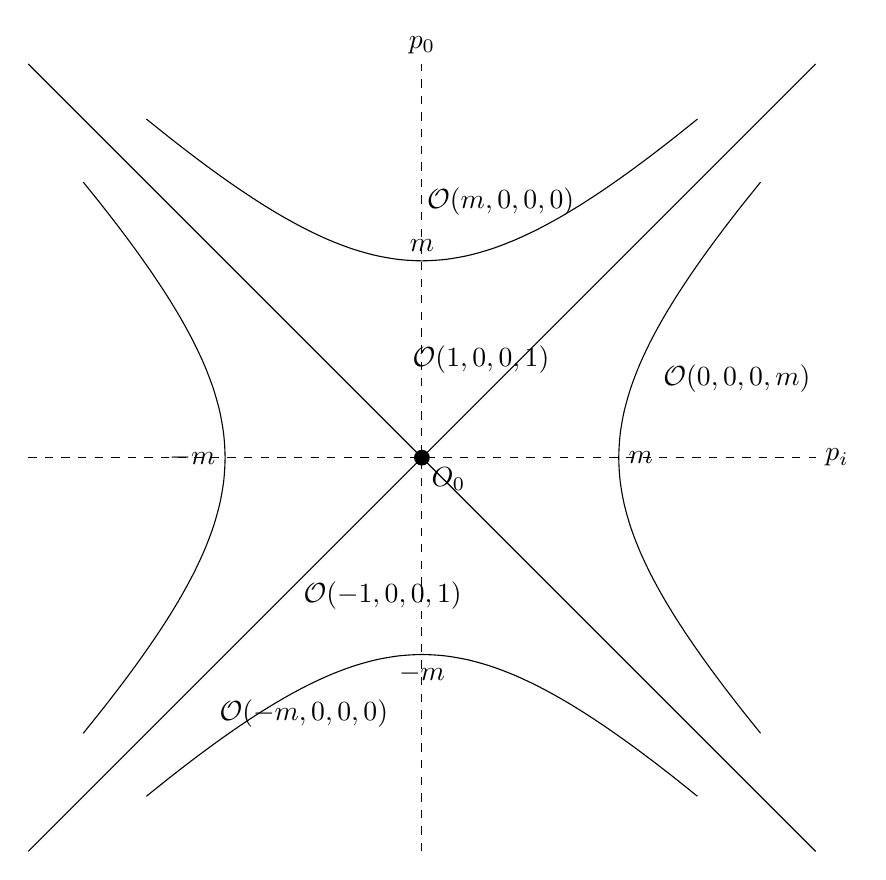
\begin{tikzpicture}[scale=2.5]
                % ===== 坐标轴 =====
                \draw[dashed] (-2,0) -- (2,0) node[right] {$p_i$};
                \draw[dashed] (0,-2) -- (0,2) node[above] {$p_0$};

                % 原点
                \fill (0,0) circle (0.04) node[below right] {$O_0$};

                % ===== 光锥 =====
                \draw (-2,-2) -- (2,2);
                \draw (-2,2) -- (2,-2);

                % ===== 质量壳：p_0^2 - p_3^2 = m^2 =====
                \draw plot[domain=-1.4:1.4,smooth,variable=\x]
                ({\x},{sqrt(\x*\x+1)});
                \draw plot[domain=-1.4:1.4,smooth,variable=\x]
                ({\x},{-sqrt(\x*\x+1)});

                % ===== 空间样轨道：p_3^2 - p_0^2 = m^2 =====
                \draw plot[domain=-1.4:1.4,smooth,variable=\x]
                ({sqrt(\x*\x+1)},{\x});
                \draw plot[domain=-1.4:1.4,smooth,variable=\x]
                ({-sqrt(\x*\x+1)},{\x});

                % ===== 标注 m, -m =====
                \node[above] at (0,1) {$m$};
                \node[below] at (0,-1) {$-m$};
                \node[right] at (1,0) {$m$};
                \node[left] at (-1,0) {$-m$};

                % ===== 轨道标记 =====
                \node at (0.4,1.3) {$\mathcal O(m,0,0,0)$};
                \node at (-0.6,-1.3) {$\mathcal O(-m,0,0,0)$};

                \node at (1.6,0.4) {$\mathcal O(0,0,0,m)$};

                \node at (0.3,0.5) {$\mathcal O(1,0,0,1)$};
                \node at (-0.2,-0.7) {$\mathcal O(-1,0,0,1)$};

                \end{tikzpicture}
                \caption{Wigner粒子分类的轨道图}
                \label{1}
                \end{figure}
\begin{center}
            \renewcommand{\arraystretch}{1.8}\label{2}
            \begin{tabular}{|c|c|c|c|c|}
            \hline
            类别
            & 四动量条件
            & 图中区域
            & 标准动量 $k^\mu$
            & 小群 $W_k$ \\ \hline

            (I) Massive
            & $p^\mu p_\mu=m^2,\; p^0>0$
            & 光锥内部（上支双曲线）
            & $(m,0,0,0)$
            & $SO(3)\simeq SU(2)$ \\ \hline

            (II) Massless
            & $p^\mu p_\mu=0,\; p^0>0$
            & 光锥本身
            & $(\kappa,0,0,\kappa)$
            & $ISO(2)$ \\ \hline

            (III) Tachyonic
            & $p^\mu p_\mu=-m^2$
            & 光锥外部（左右双曲线）
            & $(0,0,0,m)$
            & $SO(2,1)$ \\ \hline

            (IV) Trivial
            & $p^\mu=0$
            & 原点
            & $(0,0,0,0)$
            & 全洛伦兹群 \\ \hline

            \end{tabular}
\end{center}
\newpage
\subsection{正定质量粒子\(\dagger\)}


正定质量粒子（$p^2 = m^2 > 0$，$p^0 > 0$）的 Wigner 小群是三维旋转群 $SO(3)$，而为了容纳半整数自旋，必须使用其覆盖群 $SU(2)$。

在诱导表示公式 (3.13) 中，单粒子态的变换规律为：
\begin{equation}
    U(\Lambda)|\mathbf{p}, \sigma\rangle = \sqrt{\frac{(\Lambda p)^0}{p^0}} \sum_{\sigma'} D^{(j)}_{\sigma'\sigma}\{W(\Lambda, p)\}\, |(\Lambda\mathbf{p}), \sigma'\rangle
\end{equation}
其中 $W(\Lambda, p) = L^{-1}(\Lambda p)\Lambda L(p)$ 是 Wigner 旋转（一个纯粹的三维空间旋转），而 $D^{(j)}_{\sigma'\sigma}$ 是 $SU(2)$ 的 $(2j+1)$ 维不可约表示矩阵。

因此，构造有质量粒子态的全部问题归结为：\textbf{找出 $SU(2)$ 的所有有限维不可约表示}。下面利用 Lie 代数方法系统地完成这一任务。

\subsubsection*{升降算符与本征值谱}

$SU(2)$ 的 Lie 代数由三个生成元 $J_1, J_2, J_3$ 构成，满足 $[J_i, J_j] = i\epsilon_{ijk}J_k$。我们选择 $J_3$ 为对角生成元（这总是可以做到的，因为至少可以通过相似变换使一个生成元对角化），并引入升降算符：
\begin{equation}
    J_+ = \frac{1}{\sqrt{2}}(J_1 + iJ_2), \quad J_- = \frac{1}{\sqrt{2}}(J_1 - iJ_2)
\end{equation}
利用 $[J_i, J_j] = i\epsilon_{ijk}J_k$ 可以推导出升降算符满足的对易关系：
\begin{equation}
    [J_3, J_\pm] = \pm J_\pm, \quad [J_+, J_-] = J_3
\end{equation}

第一个关系 $[J_3, J_\pm] = \pm J_\pm$ 揭示了升降算符名字的来历。设 $|j, \sigma\rangle$ 是 $J_3$ 的本征态，本征值为 $\sigma$（即 $J_3|j,\sigma\rangle = \sigma|j,\sigma\rangle$），那么 $J_\pm|j,\sigma\rangle$ 仍然是 $J_3$ 的本征态，但本征值变成了 $\sigma \pm 1$：
\begin{equation}
    J_3(J_\pm|j,\sigma\rangle) = J_\pm J_3|j,\sigma\rangle + [J_3, J_\pm]|j,\sigma\rangle = \sigma J_\pm|j,\sigma\rangle \pm J_\pm|j,\sigma\rangle = (\sigma \pm 1)(J_\pm|j,\sigma\rangle)
\end{equation}
$J_+$ 将 $J_3$ 的本征值提高 $1$，$J_-$ 将其降低 $1$。

由于我们讨论的是有限维表示（表示空间的维度有限，对应的线性独立本征向量个数有限），升降过程不能无限进行。必须存在一个最大本征值 $j$ 和一个最小本征值，使得：
\begin{equation}
    J_+|j, j\rangle = 0, \quad J_-|j, -j\rangle = 0
\end{equation}

从 $|j, j\rangle$ 出发反复作用 $J_-$，经过有限步后到达 $|j, -j\rangle$。整个过程产生的本征值序列为：
\begin{equation}
    j, \; j-1, \; j-2, \; \ldots, \; -j+1, \; -j
\end{equation}
共 $2j+1$ 个值。为使序列终止于 $-j$，必须有 $2j$ 为非负整数，因此 $j$ 只能取 $0, 1/2, 1, 3/2, 2, \ldots$

\subsubsection*{Casimir 算符与表示的标记}

$SU(2)$ 恰好有一个 Casimir 算符（即与所有生成元都对易的算符）：
\begin{equation}
    \mathbf{J}^2 = J_1^2 + J_2^2 + J_3^2
\end{equation}
可以验证 $[\mathbf{J}^2, J_i] = 0$（对任意 $i$）。根据 Schur 引理，在一个不可约表示中，Casimir 算符必须正比于单位算符。

将 $\mathbf{J}^2$ 用升降算符重写为 $\mathbf{J}^2 = J_+J_- + J_-J_+ + J_3^2$，并将其作用于 $|j, \sigma\rangle$（利用升降算符的具体作用结果），经过直接计算可以得到：
\begin{equation}
    \mathbf{J}^2 |j, \sigma\rangle = j(j+1)|j, \sigma\rangle
\end{equation}
Casimir 算符的本征值 $j(j+1)$ 对于给定表示中的所有态 $|j, \sigma\rangle$（$\sigma = -j, \ldots, +j$）都相同。因此 $j$ 唯一地标记了 $SU(2)$ 的不可约表示。

\subsubsection*{低维不可约表示的显式形式}

\textbf{$j = 0$（一维表示，标量）：}

表示空间维度为 $2 \times 0 + 1 = 1$。所有生成元在这个空间中只能表示为 $1\times 1$ 的零矩阵 $J_i = 0$。群元 $U = e^{i\theta_i J_i} = e^0 = 1$。在此表示下，Lorentz 变换对态不产生任何作用——这就是自旋为 $0$ 的粒子（标量粒子）。

\textbf{$j = 1/2$（二维表示，旋量）：}

表示空间维度为 $2 \times 1/2 + 1 = 2$。$J_3$ 的本征值为 $+1/2$ 和 $-1/2$，对应本征态 $|1/2, +1/2\rangle = \binom{1}{0}$ 和 $|1/2, -1/2\rangle = \binom{0}{1}$。

生成元为 $J_i = \frac{1}{2}\sigma_i$（泡利矩阵的一半），这正是我们在第一轮中从 $SU(2)$ 的定义条件推导出的结果。群元 $U = e^{i\boldsymbol{\theta}\cdot\boldsymbol{\sigma}/2}$ 是 $2\times 2$ 幺正矩阵——它作用于二分量旋量。

这就是自旋 $1/2$ 粒子（如电子、质子、中子）的态空间。旋转 $2\pi$ 后 $U(2\pi) = -I$，态矢获得一个负号——这是半整数自旋的标志性特征。

\textbf{$j = 1$（三维表示，矢量）：}

表示空间维度为 $2 \times 1 + 1 = 3$。$J_3$ 的本征值为 $+1, 0, -1$，对应三个本征态。生成元为 $3\times 3$ 矩阵：
\begin{equation}
    J_1 = \frac{1}{\sqrt{2}}\begin{pmatrix} 0&1&0\\1&0&1\\0&1&0 \end{pmatrix}, \quad
    J_2 = \frac{1}{\sqrt{2}}\begin{pmatrix} 0&-i&0\\i&0&-i\\0&i&0 \end{pmatrix}, \quad
    J_3 = \begin{pmatrix} 1&0&0\\0&0&0\\0&0&-1 \end{pmatrix}
\end{equation}

这些生成元满足与 $SO(3)$ 的 $3\times 3$ 生成元相同的 Lie 代数——这正是因为 $SU(2)$ 的 $j=1$ 表示等价于 $SO(3)$ 的定义表示（矢量表示）。自旋为 $1$ 的粒子（如光子、$W^\pm$、$Z^0$ 玻色子）在静止系中有三个极化态。

\subsubsection*{单粒子态的完整标记}

综合 Wigner 诱导表示框架与 $SU(2)$ 的不可约表示理论，一个有质量单粒子态由以下量子数完整标记：
\begin{equation}
    |\mathbf{p}, \sigma\rangle, \quad \text{其中}\; \sigma = -j, -j+1, \ldots, +j
\end{equation}
\begin{itemize}
    \item $\mathbf{p}$：粒子的三维动量（连续量子数）。
    \item $j$：粒子的自旋（Poincaré 群第二个 Casimir 算符 $W_\mu W^\mu$ 的本征值决定），取非负整数或半整数 $j = 0, 1/2, 1, 3/2, \ldots$
    \item $\sigma$：自旋第三分量（$J_3$ 的本征值），取 $2j+1$ 个值。
\end{itemize}

粒子在一般 Lorentz 变换 $\Lambda$ 下的态变换为：
\begin{equation}
    U(\Lambda)|\mathbf{p}, \sigma\rangle = \sqrt{\frac{(\Lambda p)^0}{p^0}} \sum_{\sigma'=-j}^{+j} D^{(j)}_{\sigma'\sigma}\{W(\Lambda, p)\}\, |(\Lambda\mathbf{p}), \sigma'\rangle
\end{equation}
其中 $D^{(j)}_{\sigma'\sigma}$ 是 $SU(2)$ 自旋 $j$ 表示的 $(2j+1)\times(2j+1)$ 旋转矩阵，$W(\Lambda, p)$ 是 Wigner 旋转。

这就是有质量单粒子态的完整数学描述。关键的物理图像是：粒子的动量在 Lorentz 变换下改变（$\mathbf{p} \to \Lambda\mathbf{p}$），而自旋态在 $2j+1$ 维内部空间中进行"旋转"混合——这种混合由 Wigner 旋转通过 $SU(2)$ 表示矩阵来实现。

\subsection{零质量粒子\(\dagger\)}

对于无质量粒子（$p^\mu p_\mu = 0$，$p^0 > 0$），不存在静止参考系——粒子在任何惯性系中都以光速运动。这意味着我们不能像有质量粒子那样选取静止系四动量 $k^\mu = (m, \mathbf{0})$ 作为标准动量。

标准动量的选取改为沿 $z$ 轴传播的光子动量：
\begin{equation}
    k^\mu = (\kappa, 0, 0, \kappa)
\end{equation}
其中 $\kappa > 0$ 是一个任意的正能量参数。Wigner 小群由所有保持这个 $k^\mu$ 不变的 Lorentz 变换构成。

\subsubsection*{小群的确定：哪些 Lorentz 变换保持 $k^\mu$ 不变？}

我们需要找到所有满足 $W^\mu_{\;\nu} k^\nu = k^\mu$ 的固有正时 Lorentz 变换 $W$。

\textbf{第一类：绕 $z$ 轴的旋转 $R_z(\theta)$}

标准动量 $k^\mu = (\kappa, 0, 0, \kappa)$ 没有 $x, y$ 分量。绕 $z$ 轴旋转只混合 $x$ 和 $y$ 分量，对 $t$ 和 $z$ 分量无影响。因此 $R_z(\theta) k = k$ 对任意 $\theta$ 成立。这给出了小群的一个 $SO(2)$ 子群，由单参数 $\theta$ 描述。

\textbf{第二类：两个"异常"变换}

除了绕 $z$ 轴的旋转之外，还存在两个额外的保持 $k^\mu$ 不变的 Lorentz 变换。它们的物理图像不如旋转那么直观——它们是 Boost 和旋转的特定组合。

为了系统地找到这些变换，我们考虑无穷小情况。设 $W \approx I + \omega$，其中 $\omega^{\mu\nu}$ 是反对称的无穷小参数。条件 $W k = k$ 要求 $\omega^{\mu}_{\;\nu} k^\nu = 0$，即：
\begin{equation}
    \omega^{\mu}_{\;\nu} k^\nu = \omega^{\mu}_{\;0} \kappa + \omega^{\mu}_{\;3} \kappa = (\omega^{\mu}_{\;0} + \omega^{\mu}_{\;3})\kappa = 0
\end{equation}
这给出约束 $\omega^{\mu}_{\;0} = -\omega^{\mu}_{\;3}$。

利用 $\omega_{\mu\nu}$ 的反对称性（$\omega_{\mu\nu} = -\omega_{\nu\mu}$），独立的自由参数可以选取为三个：
\begin{itemize}
    \item $\omega_{12} = -\omega_{21}$：对应绕 $z$ 轴的旋转（即 $R_z(\theta)$），生成元为 $J_3$。
    \item $\omega_{20} + \omega_{23} = 0$ 对应的组合：定义生成元 $\Pi_1 = K_1 - J_2$（即沿 $x$ 方向的 Boost 减去绕 $y$ 轴的旋转）。
    \item $\omega_{10} + \omega_{13} = 0$ 对应的组合：定义生成元 $\Pi_2 = K_2 + J_1$（即沿 $y$ 方向的 Boost 加上绕 $x$ 轴的旋转）。
\end{itemize}

\subsubsection*{$ISO(2)$ 的 Lie 代数}

利用 Lorentz 群的对易关系（式 (3.7a)--(3.7g)），可以直接计算这三个生成元 $J_3, \Pi_1, \Pi_2$ 之间的对易关系：
\begin{align}
    [J_3, \Pi_1] &= [J_3, K_1 - J_2] = iK_2 + iJ_1 = i\Pi_2 \\
    [J_3, \Pi_2] &= [J_3, K_2 + J_1] = -iK_1 + iJ_2 = -i\Pi_1 \\
    [\Pi_1, \Pi_2] &= [K_1 - J_2, K_2 + J_1] = [K_1, K_2] + [K_1, J_1] - [J_2, K_2] - [J_2, J_1]
\end{align}
逐项利用 Lorentz 代数（$[K_i, K_j] = -i\epsilon_{ijk}J_k$，$[J_i, K_j] = i\epsilon_{ijk}K_k$，$[J_i, J_j] = i\epsilon_{ijk}J_k$）：
\begin{equation}
    [K_1, K_2] = -iJ_3, \quad [K_1, J_1] = 0, \quad [J_2, K_2] = 0, \quad [J_2, J_1] = -iJ_3
\end{equation}
因此：
\begin{equation}
    [\Pi_1, \Pi_2] = -iJ_3 + 0 - 0 - (-iJ_3) = -iJ_3 + iJ_3 = 0
\end{equation}

总结三个生成元的对易关系：
\begin{equation}
    [J_3, \Pi_1] = i\Pi_2, \quad [J_3, \Pi_2] = -i\Pi_1, \quad [\Pi_1, \Pi_2] = 0
\end{equation}

这正是\textbf{二维欧几里得群 $ISO(2)$ 的 Lie 代数}！其中 $J_3$ 是旋转生成元，$\Pi_1, \Pi_2$ 是"平移"生成元。$\Pi_1$ 和 $\Pi_2$ 之间对易（它们构成阿贝尔正规子群），而 $J_3$ 对 $\Pi_1, \Pi_2$ 的作用恰好是二维平面上的旋转。

与 $SU(2)$（Lie 代数 $[J_i, J_j] = i\epsilon_{ijk}J_k$，所有生成元不对易）相比，$ISO(2)$ 包含一个对易的"平移"部分——这使得其表示论发生了质的变化。

\subsubsection*{物理表示的选取：排除连续自旋}

$ISO(2)$ 的一般不可约表示可以用 $\Pi_1, \Pi_2$ 的本征值来标记。由于 $[\Pi_1, \Pi_2] = 0$，它们可以同时对角化。设 $\Pi_1|\psi\rangle = \pi_1|\psi\rangle$，$\Pi_2|\psi\rangle = \pi_2|\psi\rangle$。

但 $J_3$ 对 $\Pi_1, \Pi_2$ 的作用效果（由 $[J_3, \Pi_i]$ 给出）表明：$J_3$ 会将 $(\pi_1, \pi_2)$ 在二维平面内旋转，但不改变 $\pi_1^2 + \pi_2^2$ 的值。因此 $\pi_1^2 + \pi_2^2$ 是一个 Casimir 算符。

如果 $\pi_1^2 + \pi_2^2 \neq 0$，则 $J_3$ 的谱是连续的（因为 $J_3$ 的作用等价于在以 $\sqrt{\pi_1^2+\pi_2^2}$ 为半径的圆上旋转）。这样的表示称为\textbf{连续自旋表示}（continuous spin representation）。在自然界中从未观测到具有连续自旋的粒子。

因此，物理要求我们选取：
\begin{equation}
    \Pi_1 = \Pi_2 = 0
\end{equation}
即"平移"生成元的本征值为零。这个条件将 $ISO(2)$ 的表示约化为其旋转子群 $SO(2)$ 的表示。

\subsubsection*{螺旋度：$SO(2)$ 的不可约表示}

在 $\Pi_1 = \Pi_2 = 0$ 的条件下，剩余的生成元只有 $J_3$——绕动量方向的旋转。$SO(2)$ 是阿贝尔群，因此其全部不可约表示都是一维的，由 $J_3$ 的本征值 $\lambda$ 标记：
\begin{equation}
    J_3|\mathbf{k}, \lambda\rangle = \lambda|\mathbf{k}, \lambda\rangle
\end{equation}
$\lambda$ 称为\textbf{螺旋度（helicity）}——它是角动量在动量方向上的投影。

$\lambda$ 的取值范围是什么？在 $SO(2)$ 的普通表示中，$\lambda$ 可以取任意整数。但由于我们使用的是 Lorentz 群的覆盖群 $SL(2,\mathbb{C})$（这与第一轮中 $SU(2)$ 覆盖 $SO(3)$ 的逻辑完全平行），$\lambda$ 也可以取半整数值。

对于给定的无质量粒子类型（由其自旋 $j$ 标记），螺旋度只取两个值：
\begin{equation}
    \lambda = +j \quad \text{或} \quad \lambda = -j
\end{equation}
这与有质量粒子具有 $2j+1$ 个自旋投影形成了鲜明对比！

\subsubsection*{物理例子与有质量/无质量粒子的对比}

\textbf{光子（$j = 1$）：}螺旋度 $\lambda = \pm 1$，对应右旋和左旋圆偏振。纵向极化 $\lambda = 0$ 不存在——这正是为什么经典电磁波是横波。有质量的矢量玻色子（如 $W^\pm, Z^0$）则有三个极化态 $\sigma = -1, 0, +1$。

\textbf{引力子（$j = 2$，假设存在）：}螺旋度 $\lambda = \pm 2$，对应引力波的两种极化模式（$+$ 和 $\times$）。

\textbf{中微子（$j = 1/2$）：}如果中微子严格无质量，则螺旋度 $\lambda = -1/2$（左手中微子）或 $\lambda = +1/2$（右手反中微子）。实验中观测到中微子振荡表明中微子实际具有微小质量，但在高能极限下螺旋度仍然是一个极好的近似量子数。

\textbf{小群与自由度的对比表：}

\begin{center}
\renewcommand{\arraystretch}{1.4}
\begin{tabular}{c c c c c}
    \toprule
    & \textbf{标准动量 $k^\mu$} & \textbf{小群} & \textbf{内部量子数} & \textbf{自由度数} \\
    \midrule
    有质量 & $(m, \mathbf{0})$ & $SO(3) \simeq SU(2)$ & $\sigma = -j, \ldots, +j$ & $2j+1$ \\
    无质量 & $(\kappa, 0, 0, \kappa)$ & $ISO(2) \xrightarrow{\Pi=0} SO(2)$ & $\lambda = \pm j$ & $2$ \\
    \bottomrule
\end{tabular}
\end{center}

有质量粒子的内部自由度由 $SU(2)$ 的 $(2j+1)$ 维不可约表示描述，来源于粒子具有静止系——在静止系中角动量可以指向任意方向。

无质量粒子没有静止系，角动量只能沿着（或反着）动量方向——因此只有两个螺旋度 $\lambda = \pm j$。从群论角度看，这是因为 $ISO(2)$ 的物理表示被约化为其阿贝尔子群 $SO(2)$ 的一维表示。

\subsubsection*{无质量粒子态的完整变换公式}

综合以上分析，无质量单粒子态在 Lorentz 变换下的行为为：
\begin{equation}
    U(\Lambda)|\mathbf{p}, \lambda\rangle = \sqrt{\frac{(\Lambda p)^0}{p^0}}\, e^{i\lambda\theta(\Lambda, p)}\, |(\Lambda\mathbf{p}), \lambda\rangle
\end{equation}
其中 $\theta(\Lambda, p)$ 是 Wigner 旋转中绕 $z$ 轴旋转的角度（Wigner 旋转在无质量情况下退化为一个 $SO(2)$ 旋转加上物理上不可观测的 $\Pi$ "平移"）。

与有质量粒子的公式对比：
\begin{equation}
    U(\Lambda)|\mathbf{p}, \sigma\rangle = \sqrt{\frac{(\Lambda p)^0}{p^0}} \sum_{\sigma'} D^{(j)}_{\sigma'\sigma}\{W(\Lambda, p)\}\, |(\Lambda\mathbf{p}), \sigma'\rangle
\end{equation}
无质量情况中 $D$ 矩阵退化为一个相位因子 $e^{i\lambda\theta}$（$SO(2)$ 的一维表示），不再有自旋分量之间的混合——螺旋度 $\lambda$ 在 Lorentz 变换下是不变的。这是无质量粒子最显著的特征。